\section{Resource Sharing}
Resource sharing in our context refers to the ability of microfrontends to efficiently utilize and share common assets, dependencies, and services to minimize redundancy and improve performance. This is an area where our implementation is lacking the most. \\

\noindent
Although in our application each microfrontend and the application shell use the same version of most dependencies, each microfrontend still includes its own version of them. This is a tradeoff we have accepted for the strong isolation provided by Web Components. Using the Source Map Explorer package, we can analyze the space usage of our bundles through source maps. \\

\noindent
Image \ref{fig:user-usage} shows the results of running it on the \texttt{main.js} file of the \texttt{user-management} microfrontend and \ref{fig:task-usage} shows the results for the \texttt{main.js} file of the \texttt{task-management} microfrontend. In both cases, the dependencies (node\_modules) take up about 70\% of the size, while the actual code accounts for only about 30\%. Angular core dependencies take up approximately 35\% to 40\% out of the entire file size. Another significant portion is occupied by the \texttt{chart.js} library, which we use for creating graphs for the dashboard, contributing around 20\%. The remaining dependencies can be considered negligible. \\
\begin{figure}[h]
    \centerline{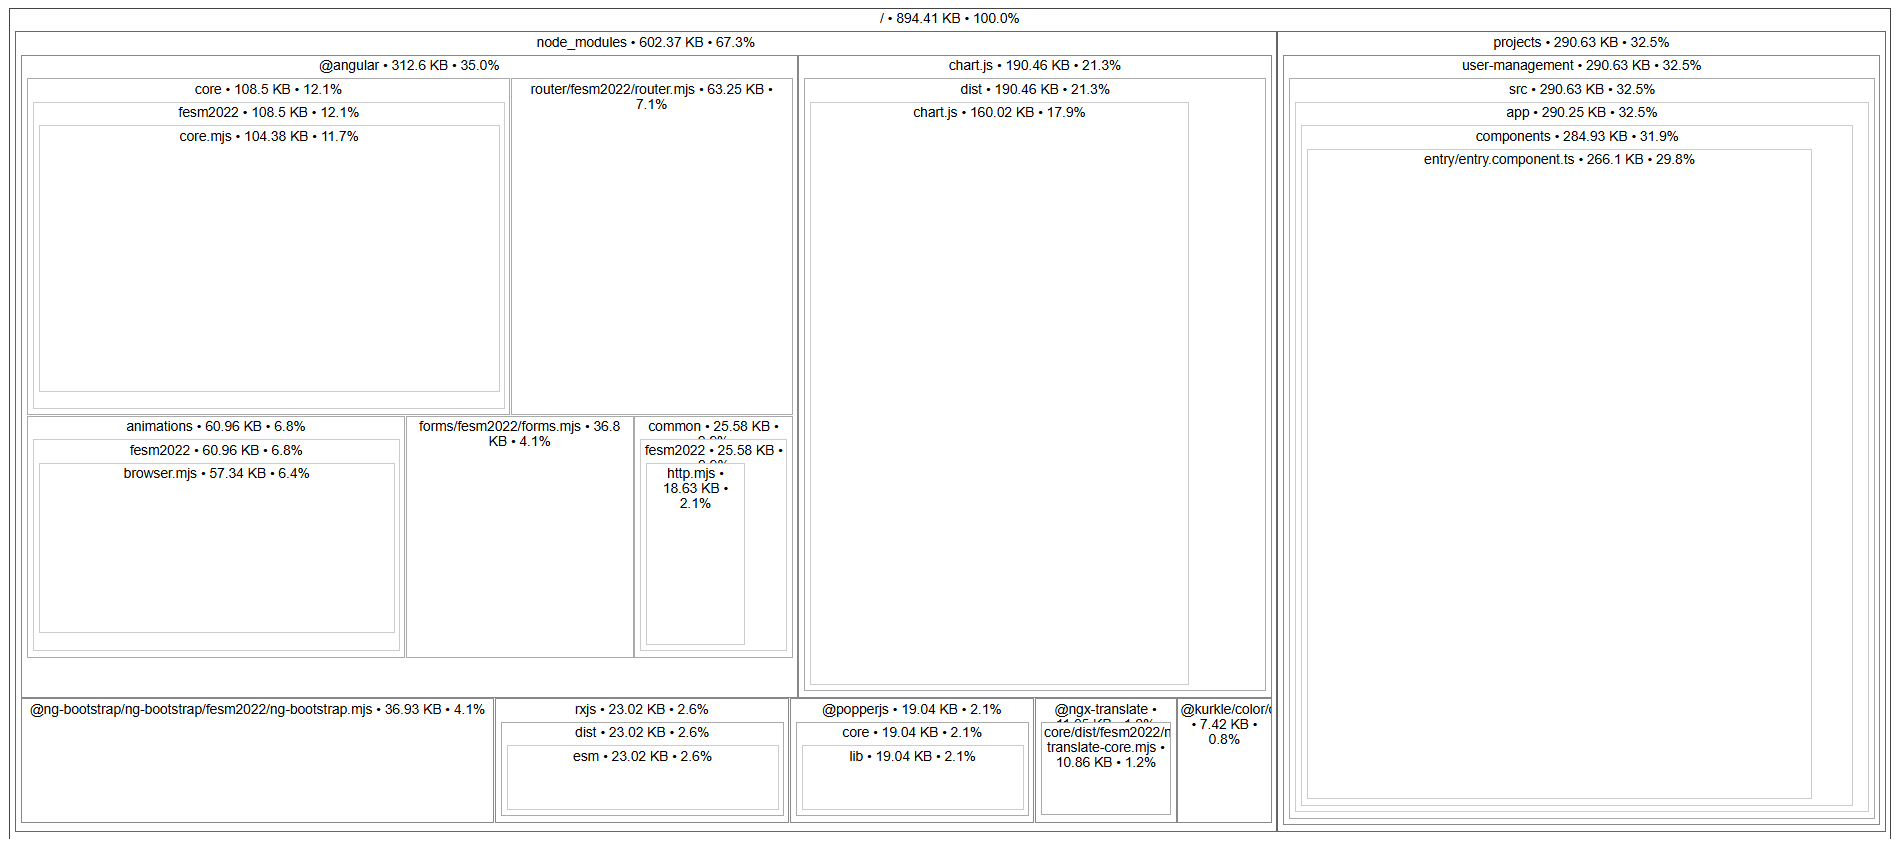
\includegraphics[width=1\textwidth]{images/user-space-usage.png}}
    \caption[Space usage of the user-management microfrontend]{Space usage of the \texttt{main.js} file in the user-management microfrontend}
    \label{fig:user-usage} 
\end{figure}

\begin{figure}[h]
    \centerline{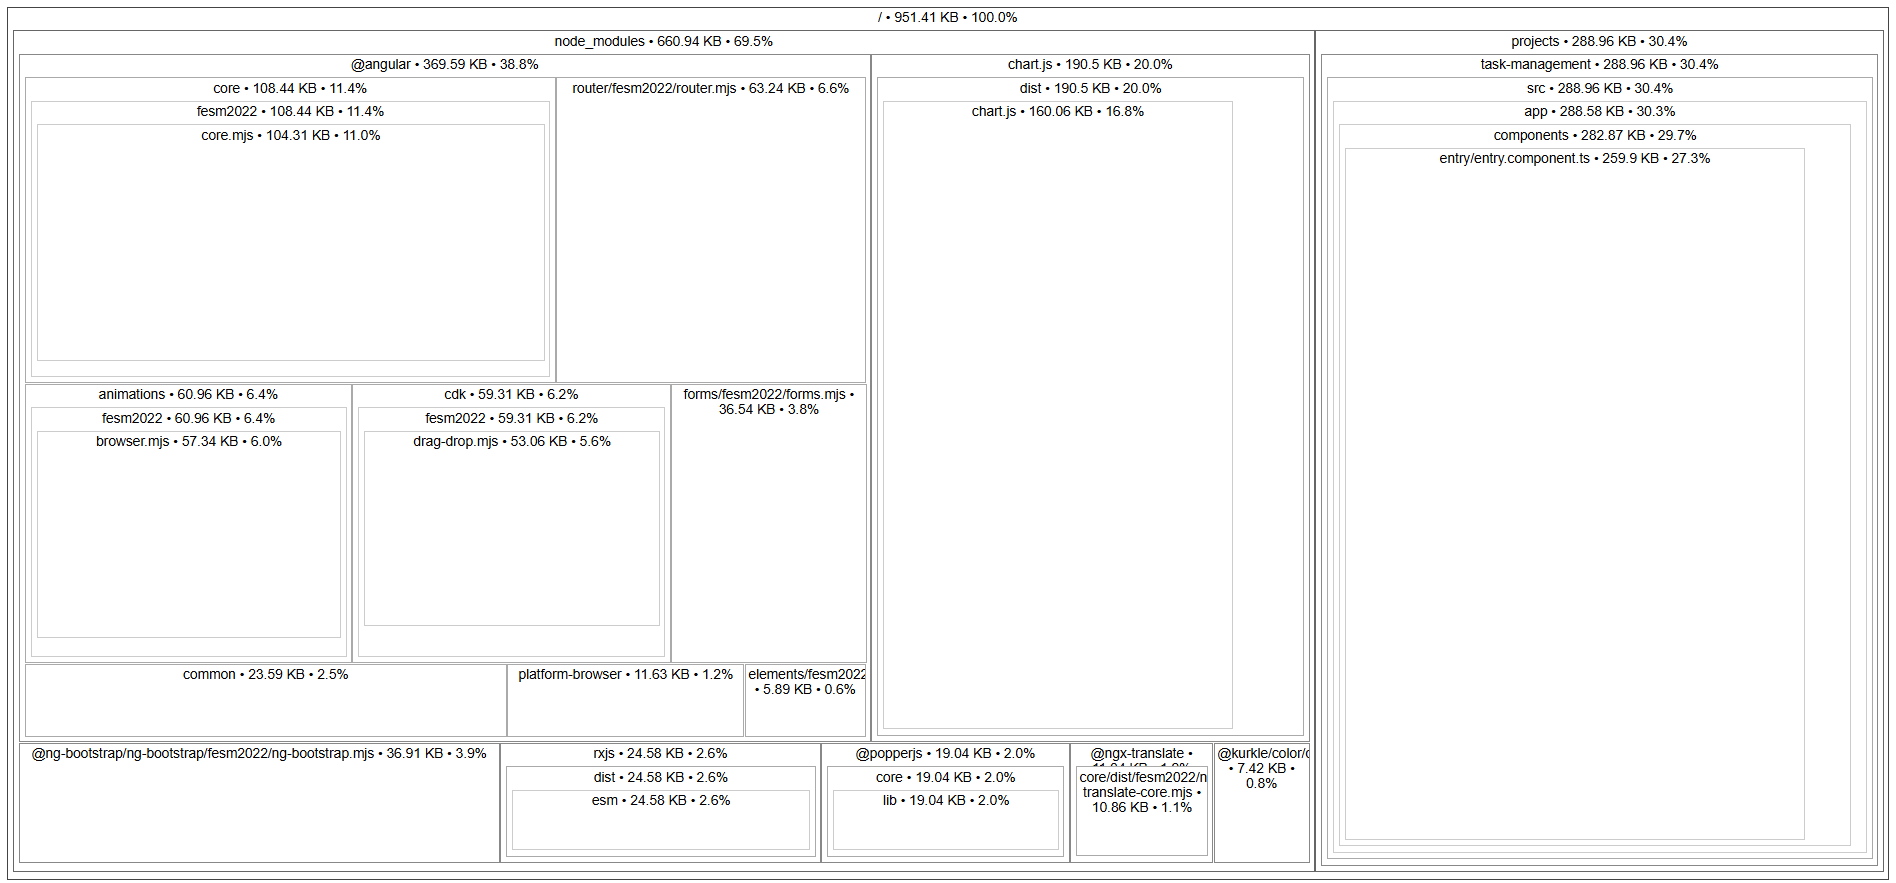
\includegraphics[width=1\textwidth]{images/task-space-usage.png}}
    \caption[Space usage of the task-management microfrontend]{Space usage of the \texttt{main.js} file in the task-management microfrontend}
    \label{fig:task-usage} 
\end{figure}
\noindent
Based on this analysis, we can conclude that our application would significantly benefit from sharing Angular core dependencies across the microfrontends and potentially also the \texttt{chart.js} library. However, we were unable to focus on this issue due to time limitations. One potential solution is combining the Web Components approach with the Module Federation Webpack plugin, especially since we are already using Webpack.